\subsection{LLMs as Optimizers} \label{sec:llm-optimizers}

\begin{figure}[htb]
    \centering
    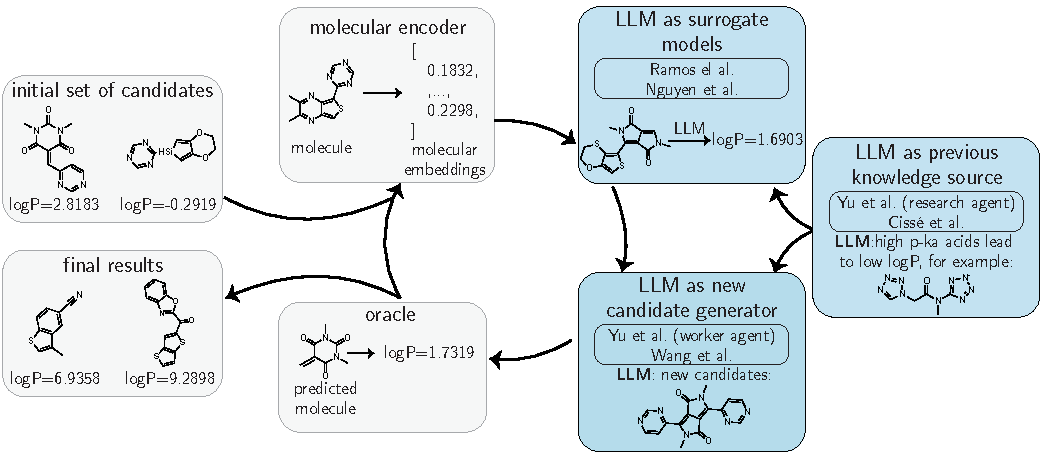
\includegraphics[width=1\textwidth]{figures/rescaled_figures/chemrev_figure22.pdf}
    \caption{\textbf{Overview of the iterative optimization loop that mirrors the structure of the optimization section}. The blue boxes contain the different roles that the \glspl{llm} play in the loop, and which are described in the main text. References in which the use of \glspl{llm} for that step are detailed inside the small boxes inside each of the components of the loop. The example shown is about obtaining molecules with high \texttt{logP}.}
    \label{fig:optimization}
\end{figure}

Discovering novel compounds and reactions in chemistry and materials science has long relied on iterative trial-and-error processes rooted in existing domain knowledge \autocite{Taylor2023brief}. While, as explained in \Cref{sec:retrosynthesis}, those methods are used to accelerate this process, optimization methods help improve conditions, binding affinity, etc.
But these approaches are slow and labor-intensive. 
Traditional data-driven methods aimed to address these limitations by combining predictive \gls{ml} models with optimization frameworks such as \gls{bo} or \glspl{ea}. 
These frameworks balance exploration of uncharted regions in chemical space with exploitation of known high-performing regions \autocite{Li2024sequential, Hse2021gryffin, Shields2021bayesian, Griffiths2020constrained, RajabiKochi2025adaptive}.

Recent advances in \glspl{llm} have unlocked potential for addressing optimization challenges in chemistry and related domains \autocite{fernando2023promptbreeder0, yang2023large, chen2024instruct}. 
A key strength of \glspl{llm} lies in their capacity to frame optimization tasks through natural language, which enhances knowledge incorporation, improves candidate comparisons, and increases interpretability. 
This aligns well with chemical problem-solving, where complex phenomena, such as reaction pathways or material behaviors, are often poorly captured by standard nomenclature; however, they can still be intuitively explained through natural language. 
Moreover, \glspl{gpm}' general capabilities provide flexibility beyond classical methods, which have to be trained from scratch if the optimization problem or any of its variables changes.
By encoding domain-specific knowledge---including reaction rules, thermodynamic principles, and structure-property relationships---into structured prompts, \glspl{llm} can synergize expertise with their ability to navigate complex chemical optimization problems.

Current \gls{llm} applications in chemistry optimization vary in scope and methodology. 
Many studies integrate \glspl{llm} into \gls{bo} frameworks, where models guide experimental design by predicting promising candidates \autocite{rankovic2023bochemian}. Others employ \glspl{ga} or hybrid strategies that combine \gls{llm}-generated hypotheses with computational screening \autocite{cisse2025language0based}.  

\subsubsection{LLMs as Surrogate Models}

A prominent \gls{llm}-driven strategy positions these models as surrogate models within optimization loops. Typically implemented as \gls{gpr}, surrogate models learn from prior data to approximate costly feature-outcome landscapes, which are often computationally and time-consuming to evaluate, thereby guiding the acquisition.
\glspl{llm} offer major advantages in this role primarily through strong low-data performance. 
Their \gls{icl} capability enables task demonstration with minimal prompt examples while leveraging chemical knowledge from pre-training to generate accurate predictions. 
This allows \glspl{gpm} to compensate for sparse experimental data effectively.

\textcite{ramos2023bayesian} demonstrated the viability of this paradigm through a simple yet effective framework that combines \gls{icl} using only one example in the prompt with a \gls{bo} workflow. 
Their \gls{bo}-\gls{icl} approach uses few-shot examples formatted as question-answer pairs, where the \gls{llm} generates candidate solutions conditioned on prior successful iterations. 
These candidates are ranked using an acquisition function, with top-$k$ selections integrated into subsequent prompts to refine predictions iteratively. 
Remarkably, this method achieved high performance in optimizing catalytic reaction conditions, even matching the top-1 accuracies observed in experimental benchmarks. This emphasizes the potential of \glspl{llm} as accessible, \gls{icl} optimizers when coupled with well-designed prompts.

To address limitations in base \glspl{llm}’ inherent chemical knowledge---particularly their grasp of specialized representations like \gls{smiles} or structure-property mappings---\textcite{yu2025collaborative} introduced a hybrid architecture augmenting pre-trained \glspl{llm} with task-specific embedding and prediction layers. 
These layers, fine-tuned on domain data, align latent representations of input-output pairs (denoted as \texttt{<x>} and \texttt{<y>} in prompts), enabling the model to map chemical structures and properties into a unified, interpretable space. Crucially, the added layers enhance chemical reasoning without sacrificing the flexibility of \gls{icl}, allowing the system to adapt to trends across iterations, similarly to what was done by \textcite{ramos2023bayesian}. 
In their evaluations of molecular optimization benchmarks, such as the \gls{pmo} \autocite{gao2022sample}, they revealed improvements over conventional methods, including \gls{bo}-\gls{gp}, \gls{rl} methods, and \gls{ga}.

\textcite{yu2025collaborative} further highlighted the framework’s extensibility to diverse black-box optimization challenges beyond chemistry. 
This represents one of the most important advantages of using \glspl{llm} as orchestrators of the optimization process. 
The flexibility of natural language in this process enables the procedure to be applied to any optimization process. 
In contrast, classical methods are constrained to the specific task for which they are designed due to the need to train the surrogate model.

\subsubsection{LLMs as Next Candidate Generators}

Recent studies demonstrate the potential of \glspl{llm} to enhance \glspl{ea} \autocite{lu2024generative} and \gls{bo} \autocite{amin2025towards} frameworks by leveraging their embedded chemical knowledge and ability to integrate prior information, thereby reducing computational effort while improving output quality.
Within \glspl{ea}, \glspl{llm} refine molecular candidates through mutations (modifying molecular substructures) or crossovers (combining parent molecules). 
In \gls{bo} frameworks, they serve as acquisition functions, utilizing surrogate model predictions---both mean and uncertainty---to select optimal molecules or reaction conditions for evaluation.

For molecule optimization, \textcite{yu2025collaborative} introduced \modelname{MultiModel}, a dual-\gls{llm} system where one model proposes candidates and the other supplies domain knowledge (see \Cref{sec:opt-llm-know-source}). 
By fine-tuning the \enquote{worker} \gls{llm} to recognize molecular scaffolds and target properties, and expanding the training pool to include a million-size pre-training dataset, they achieved hit rates exceeding $90\%$. 
Similarly, \textcite{wang2024efficient} developed \modelname{MoLLEO}, integrating an \gls{llm} into an \gls{ea} to replace random mutations with \gls{llm}-guided modifications. Here, \modelname{GPT-4} generated optimized offspring from parent molecules, significantly accelerating convergence to high fitness scores. 
Notably, while domain-specialized models (\modelname{BioT5}, \modelname{MoleculeSTM}) underperformed, the general-purpose \modelname{GPT-4} excelled---a finding that underscores the context-dependent utility of \glspl{llm}

In a related approach, \textcite{lu2024generative} showed that well-designed prompts---incorporating task-specific constraints, objectives, and few-shot examples---enable general \glspl{llm} (\modelname{Claude\--3.5-Sonnet}, \modelname{o1-preview}) to generate high-quality candidates without fine-tuning, outperforming both random selection and vanilla \glspl{ga} in functional \gls{tmc} design.

\subsubsection{LLMs as Prior Knowledge Sources} \label{sec:opt-llm-know-source}

A key advantage of integrating \glspl{llm} into optimization frameworks is their ability to encode and deploy prior knowledge within the optimization loop. 
As illustrated in \Cref{fig:optimization}, this knowledge can be directed into either the surrogate model or candidate generation module, significantly reducing the number of optimization steps required through high-quality guidance.

For example, \textcite{yu2025collaborative} deployed a \enquote{research} agent that leverages \modelname{Google} search and \modelname{RDKit} to verify and rank molecules generated by \enquote{worker} agents against target features and properties. 
Their results demonstrate substantial improvements when this filtering mechanism is applied.

Similarly, \textcite{cisse2025language0based} introduced \modelname{BORA}, which contextualizes conventional black-box \gls{bo} using an \gls{llm}. \modelname{BORA} maintains standard \gls{bo} as the core driver but strategically activates the \gls{llm} when progress stalls. 
This leverages the model’s \gls{icl} capabilities to hypothesize promising search regions and propose new samples, regulated by a lightweight heuristic policy that manages costs and incorporates domain knowledge (or user input). 
Evaluations on synthetic benchmarks such as the catalyst optimization task for hydrogen generation show that \modelname{BORA} accelerates exploration, improves convergence, and outperforms existing \gls{llm}-\gls{bo} hybrids.

To enhance the task-specific knowledge of the \gls{llm} generating feedback, \textcite{zhang2025large} fine-tuned a \modelname{Llama-2-7B} model using a multitask \gls{qa} dataset. This dataset was created with instructions from \modelname{GPT-4}. 
The resulting model served as a human assistant or operated within an active learning loop, thereby accelerating the exploration of new reaction spaces (see \Cref{sec:retrosynthesis}). 
However, as the authors note, even this task-specialized \glspl{llm} produces suboptimal suggestions for optimization tasks. 
They remain prone to hallucination and cannot assist with unreported reactions, but still, they improve for most of the applications, using pure classical methods.

\subsubsection{How to Face Optimization Problems?}

Published works explore different ways of using \glspl{llm} for optimization problems in chemistry, from simple approaches, such as just prompting the model with some initial random set of experimental candidates and iterating \autocite{ramos2023bayesian}, to fine-tuning models in \gls{bo} fashion \autocite{rankovic2025gollum0}. 
The most efficient initial point is by relying entirely on a \gls{icl} approach, which allows one to obtain a first signal rapidly. 
Such initial results will enable to determine whether a more complex, computationally intensive approach is necessary or whether prompt engineering is reliable enough for the application. 
Fine-tuning can be used as a way to enhance the chemical knowledge of the \glspl{llm} and can lead to improvements in optimization tasks where the model requires such knowledge to choose or generate better candidates. 
Fine-tuning might not be a game-changer for other approaches that rely more on sampling methods \autocite{wang2025llm0augmented}.

While some initial works showed that \glspl{llm} trained specifically on chemistry perform better for optimization tasks \autocite{kristiadi2024sober}, other works showed that a \gls{gpm} such as \modelname{GPT-4} combined with an \gls{ea} outperformed all other models \autocite{wang2024efficient}.
Is it better to incorporate a general model or a chemistry \gls{lm} into the optimization frameworks?
We hypothesize that for models of the same size (in number of parameters) and similar training size---attending to \glspl{pflop}---a chemical \gls{lm} (a specialized model) will consistently outperform general models. 
If the models differ significantly in size, the larger model will typically perform better.
